\documentclass[../AnalysisNoteJBuxton.tex]{subfiles}
\begin{document}

\subsection{Results: \texorpdfstring{$\Xi$K$^{\pm}$}{TEXT}}
\label{ResultsXiK}

Even without any fits to the data, the fact that the $\Xi^{-}$K$^{+}$ data dips below unity (Fig. \ref{fig:XiKchwConjResults}) is exciting, as this cannot occur purely from a Coulomb interaction.  We hope that this dip signifies that we are able to peer through the overwhelming contribution from the Coulomb interaction to see the effects arising from the strong interaction.

\begin{figure}[h]
  \centering
  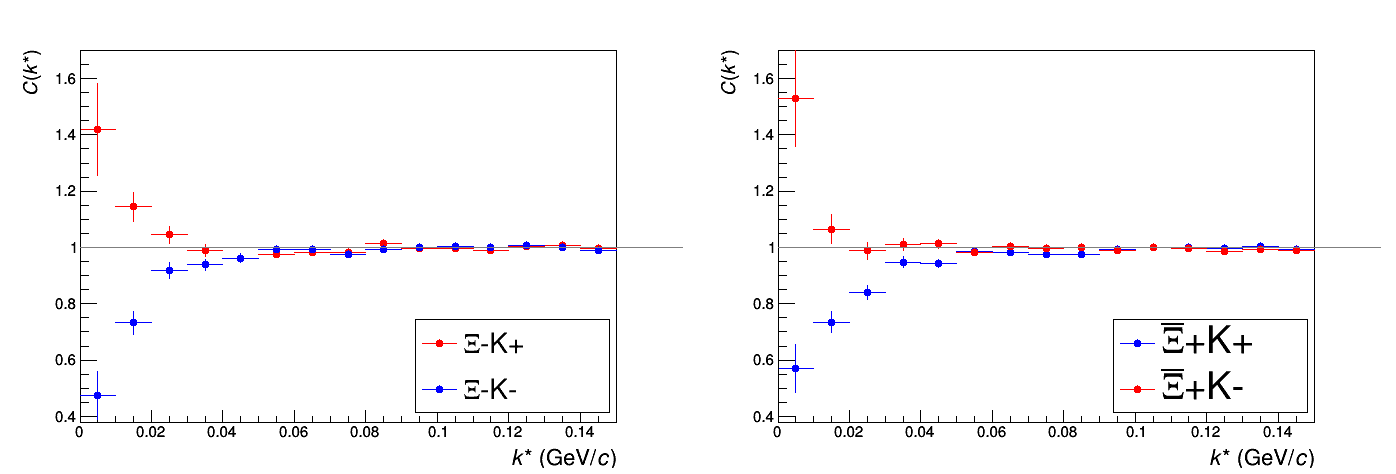
\includegraphics[width=\textwidth]{7_ResultsAndDiscussion/Figures/cXicKchKStarCfs.png}
  \caption[$\Xi$K$^{\pm}$ Results]{$\Xi$K$^{\pm}$ Results for 0-10\% Centrality.  (Left) $\Xi^{-}$K$^{+}$ and  $\Xi^{-}$K$^{-}$  (Right) $\bar{\Xi}^{+}$K$^{+}$ and  $\bar{\Xi}^{+}$K$^{-}$}
  \label{fig:XiKchwConjResults}
\end{figure}

%%%%%%%%%%%%%%%%%%%%%%%%%%%%%%%%%%%%%%%%%%%%%%%%%%%%%%%%%%%%%%%%%%%%%%%%%%%%%%%%%%%%%%%%
\begin{comment}
\begin{figure}[h!]
  \centering
  %%----start of first subfigure---  
  \subfloat[$\Xi$K$^{+}$ First Fit, 0-10\% Centrality]{
    \label{fig:XiKchFits:a}
    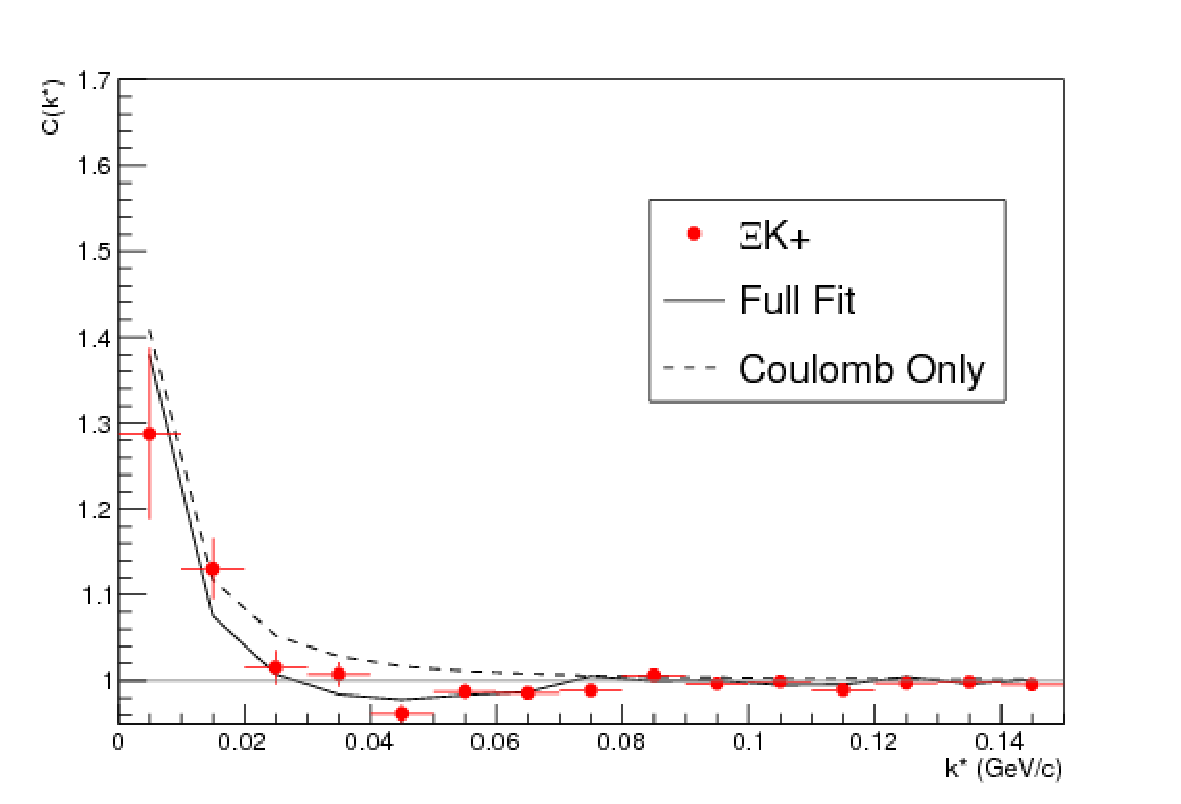
\includegraphics[width=0.49\textwidth]{7_ResultsAndDiscussion/Figures/XiKchP.pdf}}
  %%----start of second subfigure---
  \subfloat[$\bar{\Xi}$K$^{+}$ First Fit, 0-10\% Centrality]{
    \label{fig:XiKchFits:b}
    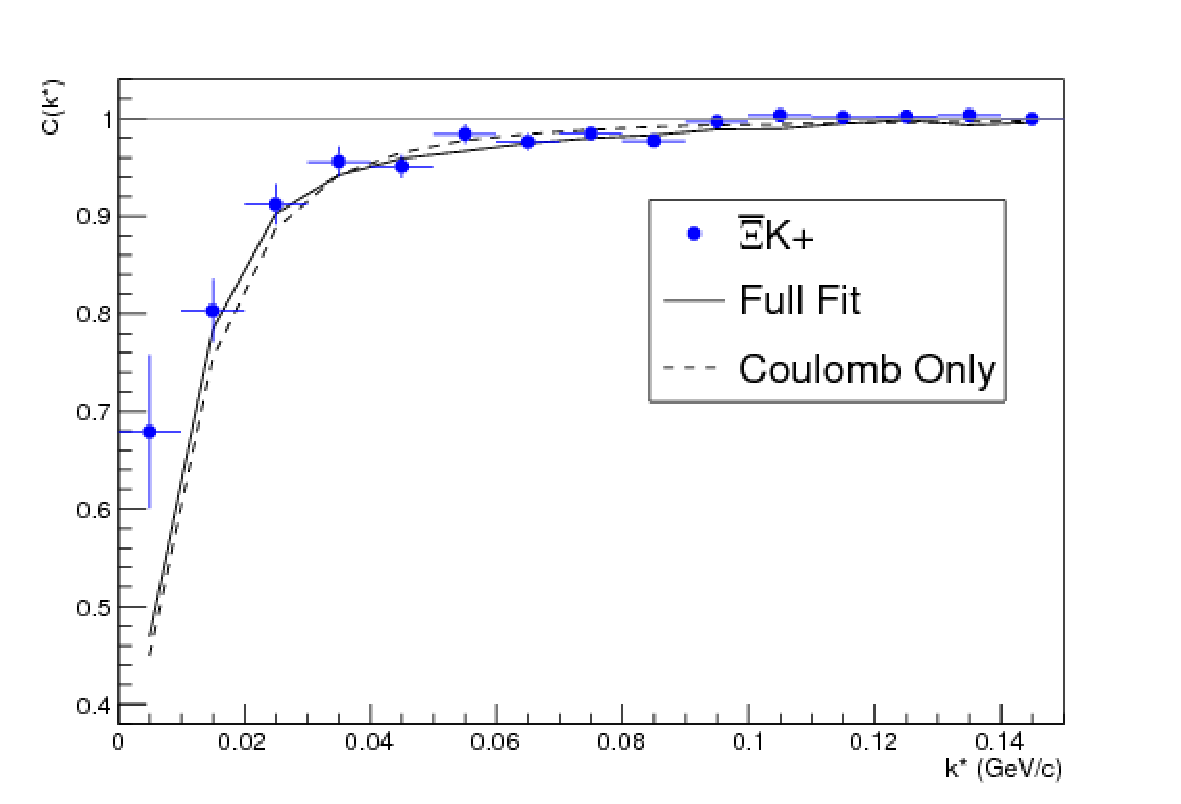
\includegraphics[width=0.49\textwidth]{7_ResultsAndDiscussion/Figures/AXiKchP.pdf}}
  %%----overall caption----
  \caption[$\Xi$K$^{\pm}$ First Fits]{$\Xi$K$^{\pm}$ First Fits}
  \label{fig:XiKchFits}
\end{figure}
\end{comment}
%%%%%%%%%%%%%%%%%%%%%%%%%%%%%%%%%%%%%%%%%%%%%%%%%%%%%%%%%%%%%%%%%%%%%%%%%%%%%%%%%%%%%%%%

Figure \ref{fig:XiKchCoulombOnlyBand} demonstrates graphically, that the $\Xi^{-}$K$^{+}$ results cannot be described by solely the Coulomb interaction.  In this figure, we present the data along with a Coulomb-only band.  The Coulomb-only band is spanned by two Coulomb-only curves, whose parameters are given in the figure. The Coulomb-only curves were generated using a technique identical to the generation of the fit function, described in Sec. \ref{ModelCascadeKaon}, except, of course, with the nuclear scattering parameters all set to zero.  The Coulomb-only curves change monotonically with varying $\lambda$ or varyin radius parametres, therefore, any curves built with parameter sets intermediate to those use in the Coulomb-only band will be contained in the band.

Including the strong interaction into the simulation can dramatically change the resulting correlation function, as shown in Figure \ref{fig:XiKchStrongInfluence}.


\begin{figure}[h]
  \centering
  %%----start of first subfigure---  
  \subfloat[$\Xi$K$^{+}$ and $\bar{\Xi}$K$^{-}$]{
    \label{fig:XiKchCoulombOnlyBand:a}
    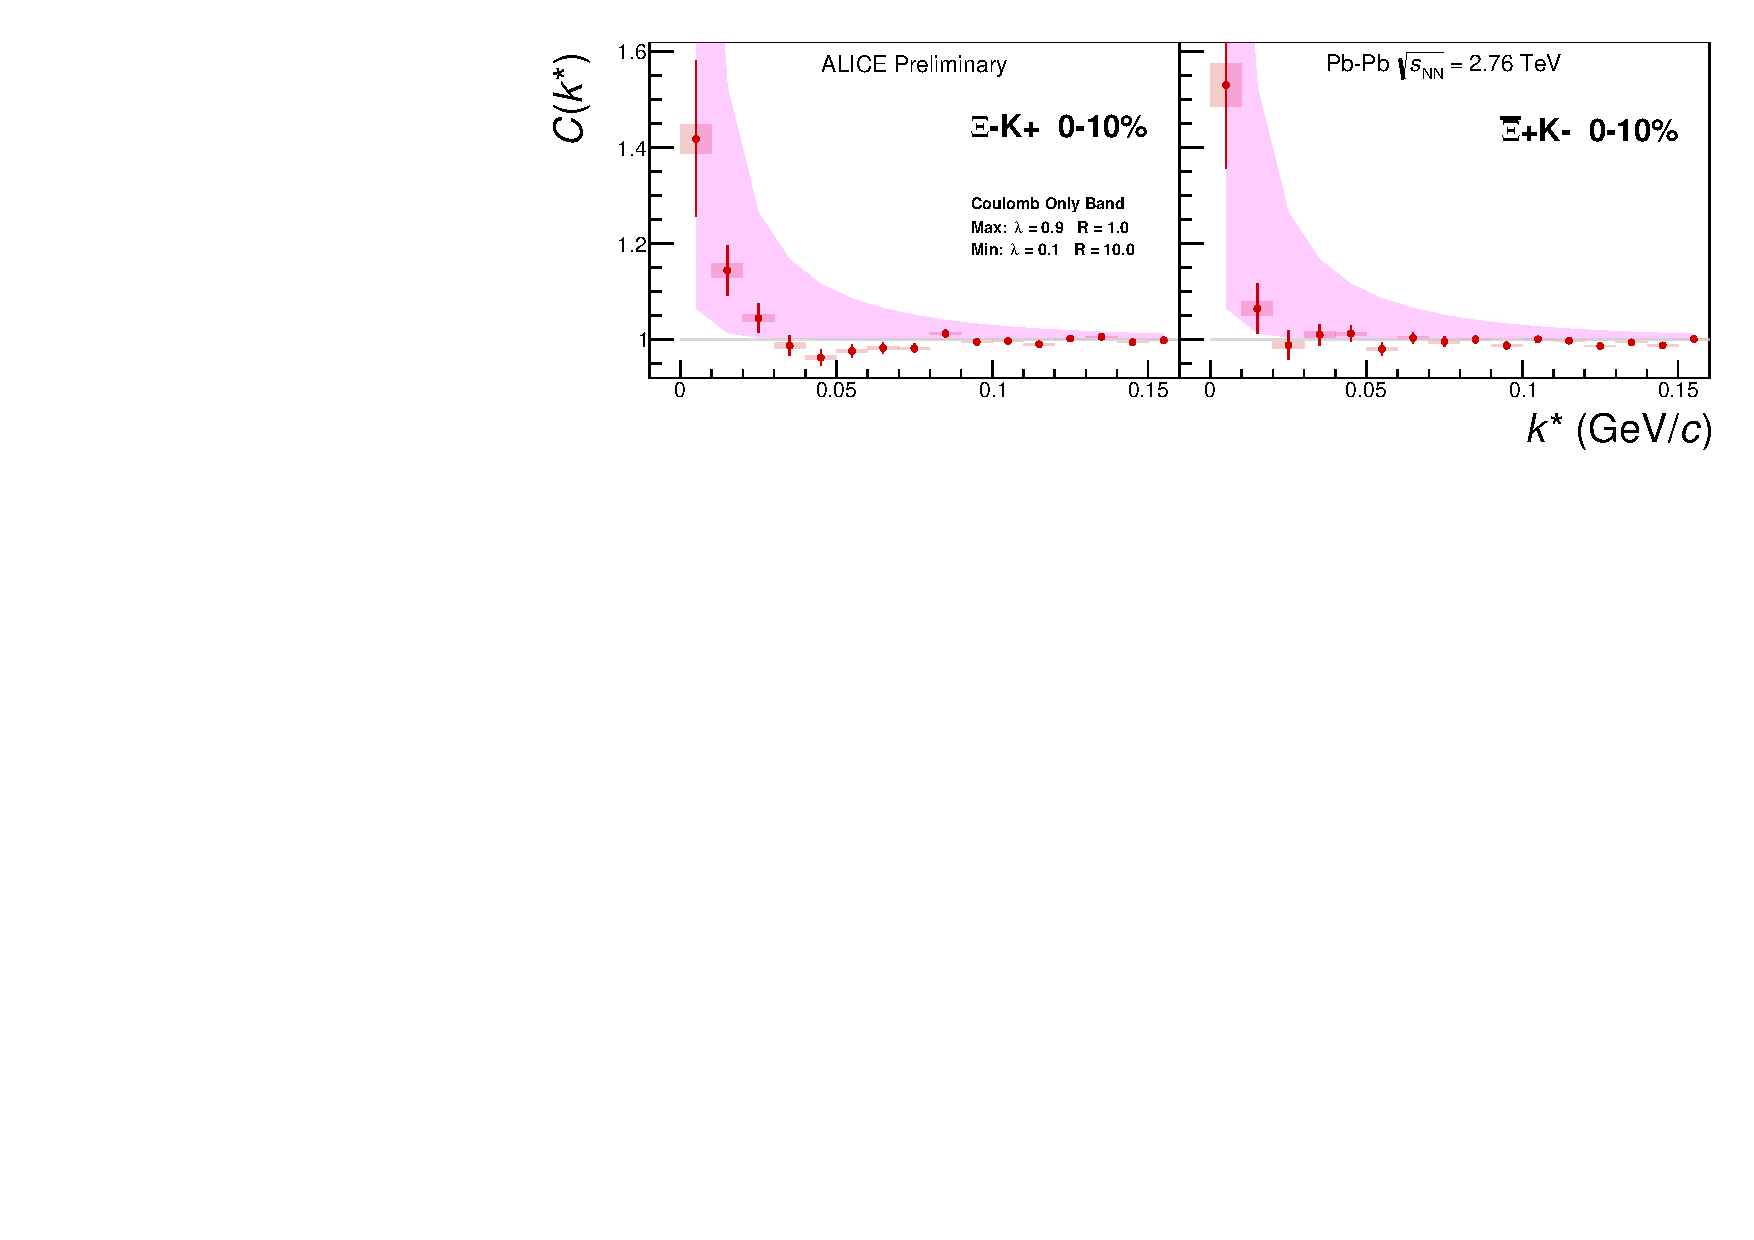
\includegraphics[width=0.99\textwidth]{7_ResultsAndDiscussion/Figures/WPCFCoulombOnlyCurves_XiKchP_0010_Stretch.pdf}}\\
  %%----start of second subfigure---
  \subfloat[$\Xi$K$^{-}$ and $\bar{\Xi}$K$^{+}$]{
    \label{fig:XiKchCoulombOnlyBand:b}
    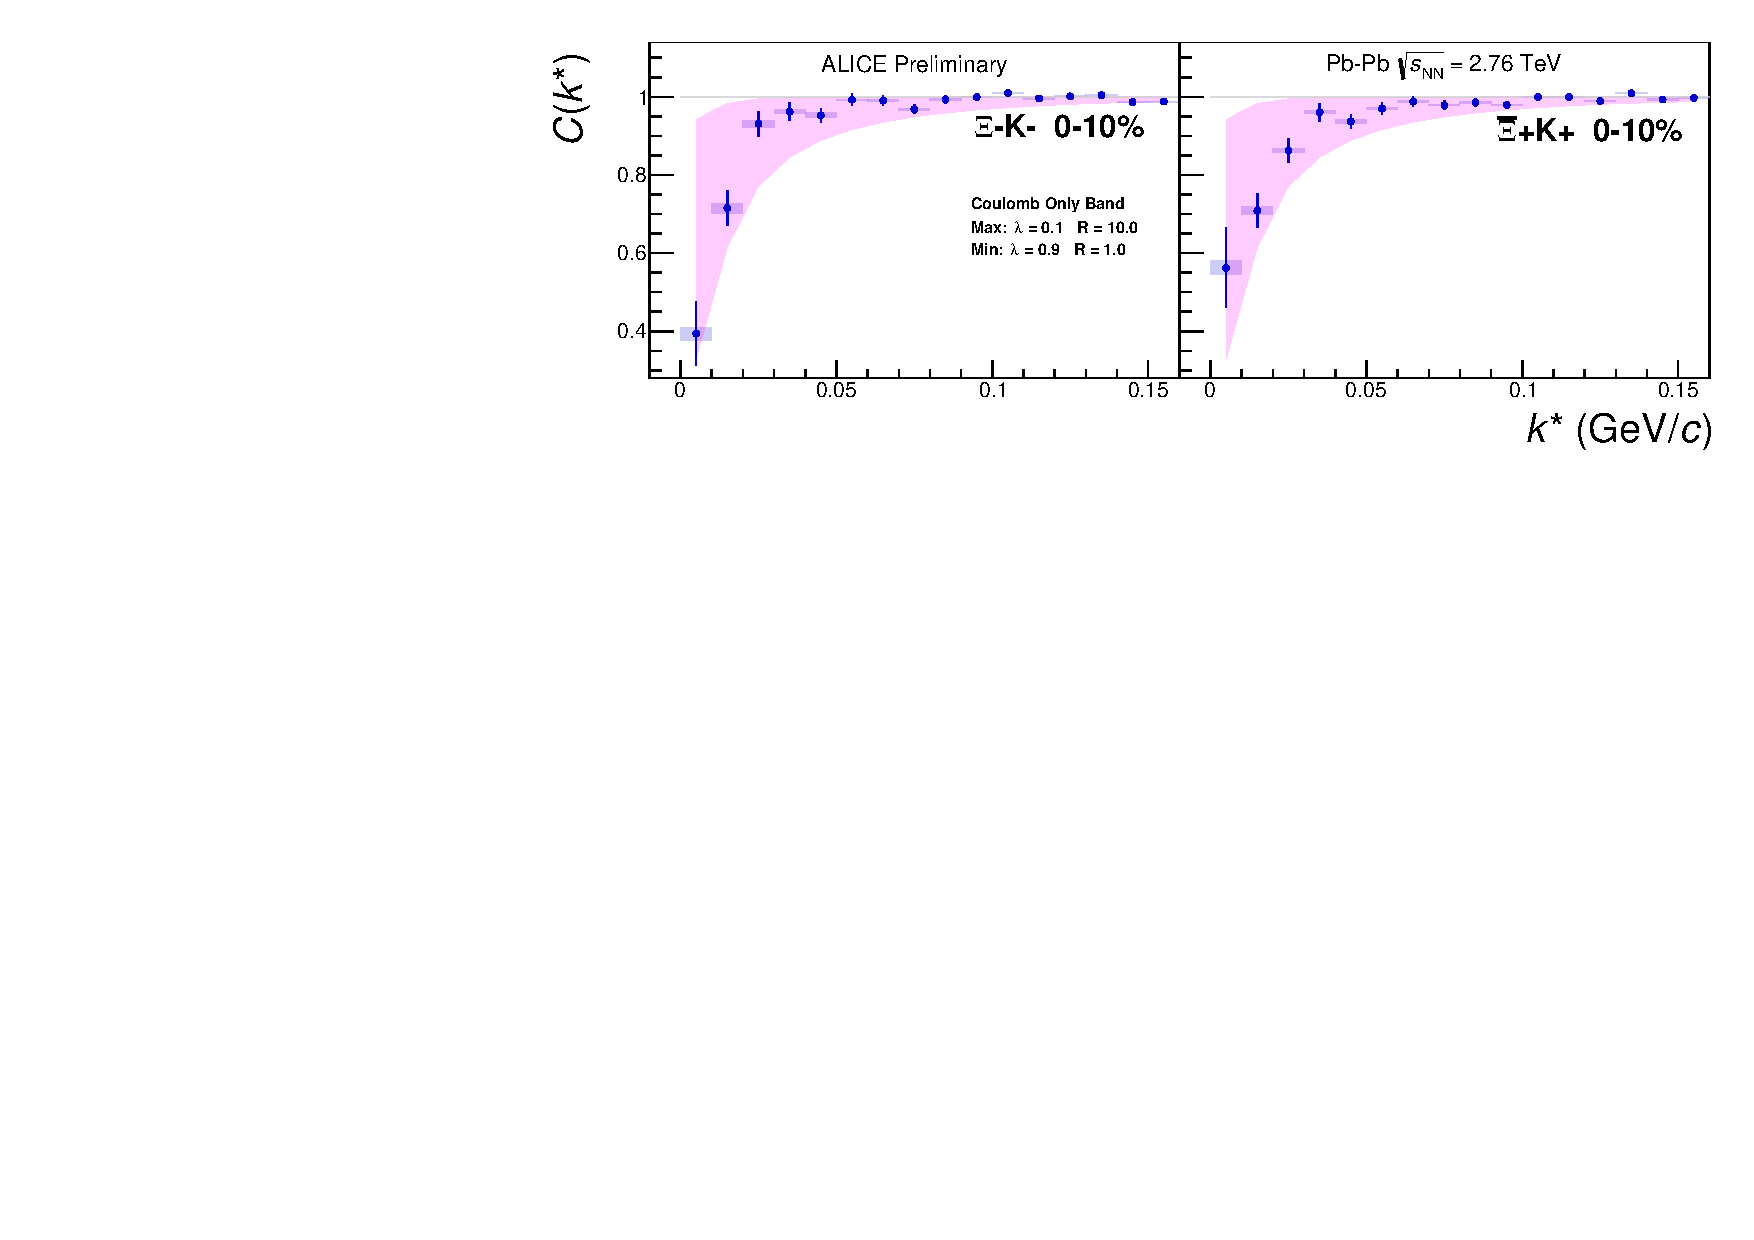
\includegraphics[width=0.99\textwidth]{7_ResultsAndDiscussion/Figures/WPCFCoulombOnlyCurves_XiKchM_0010_Stretch.pdf}}
  %%----overall caption----
  \caption[$\Xi$K$^{\pm}$ Coulomb Only Band]{$\Xi$K$^{\pm}$ Coulomb Only Band, 0-10\% Centrality}
  \label{fig:XiKchCoulombOnlyBand}
\end{figure}

\begin{figure}[h]
  \centering
  %%----start of first subfigure---  
  \subfloat[$\Xi$K$^{+}$ and $\bar{\Xi}$K$^{-}$]{
    \label{fig:XiKchStrongInfluence:a}
    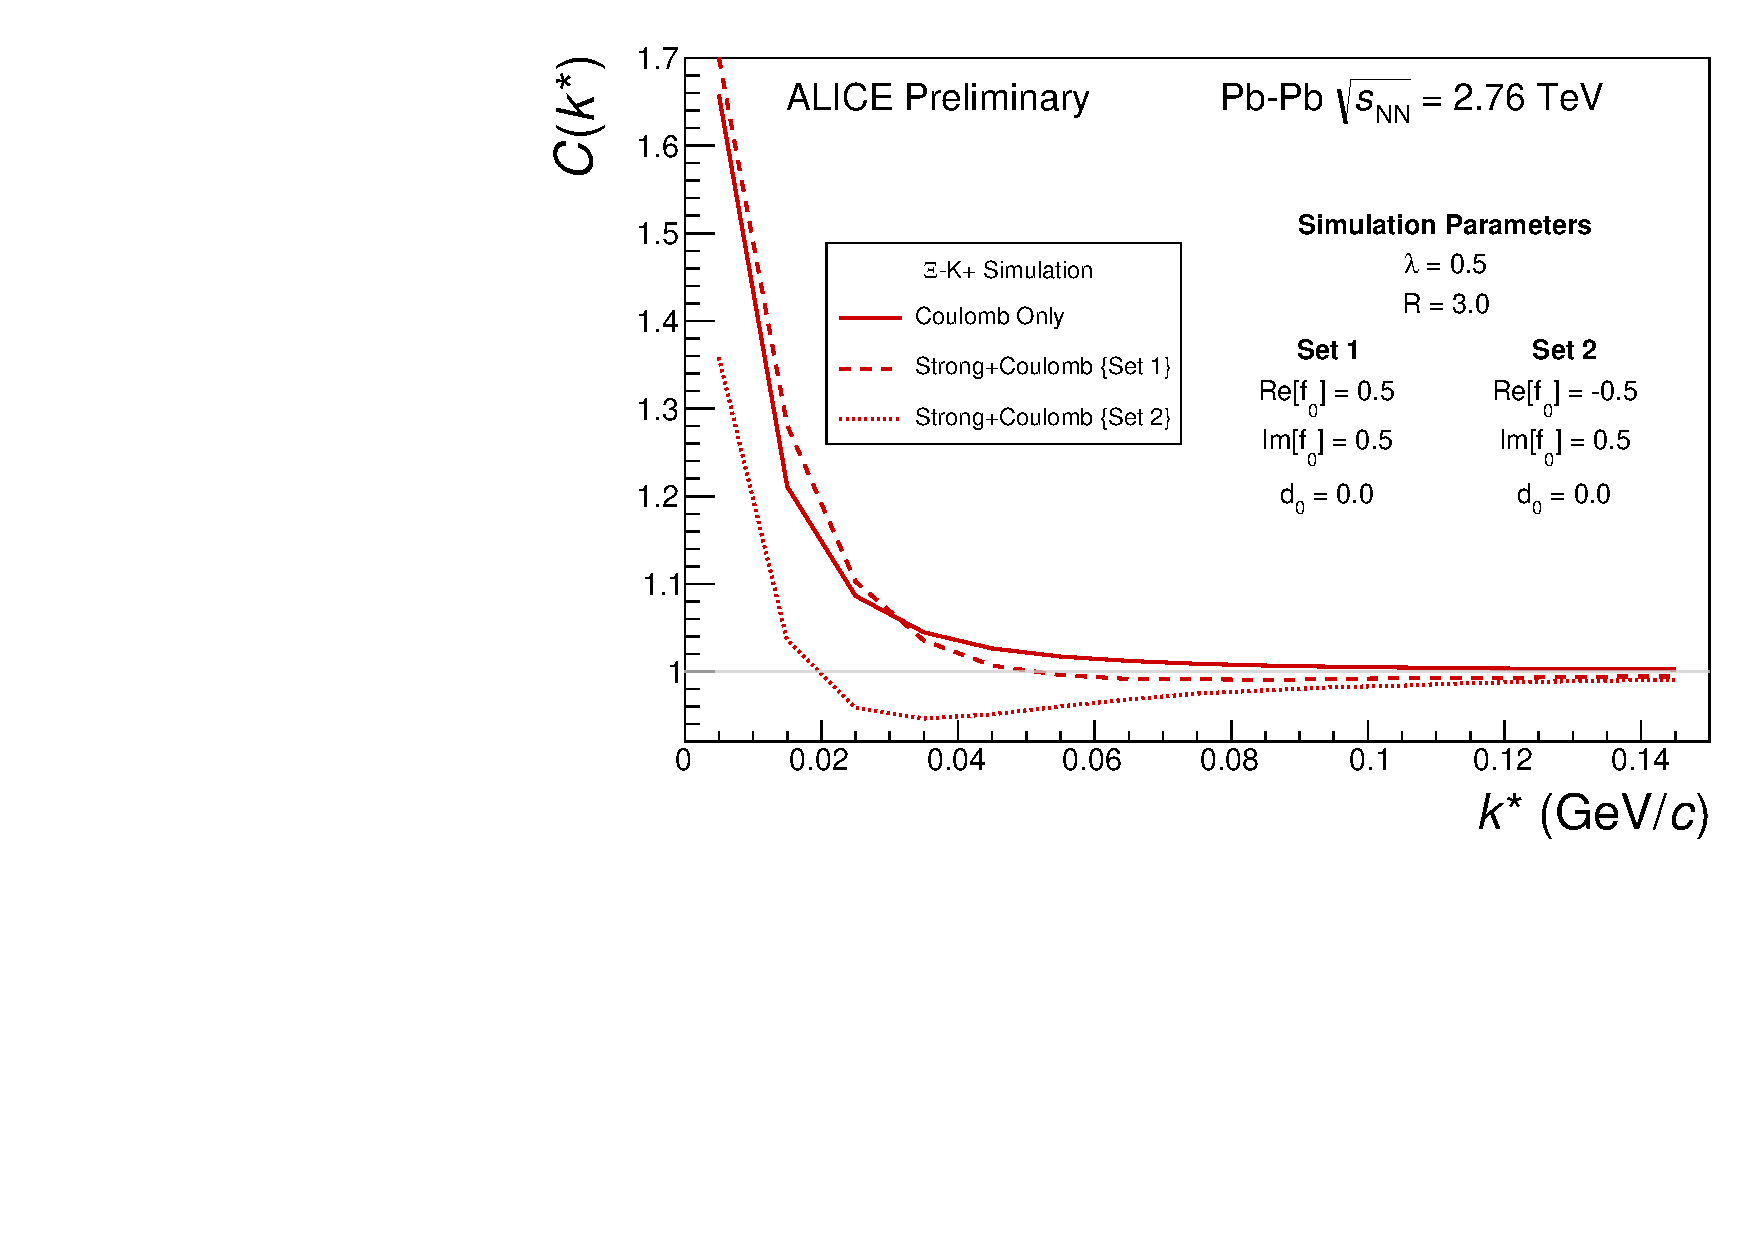
\includegraphics[width=0.99\textwidth]{7_ResultsAndDiscussion/Figures/WPCFStrongInfluence_XiKchP_0010_v2.pdf}}\\
  %%----start of second subfigure---
  \subfloat[$\Xi$K$^{-}$ and $\bar{\Xi}$K$^{+}$]{
    \label{fig:XiKchStrongInfluence:b}
    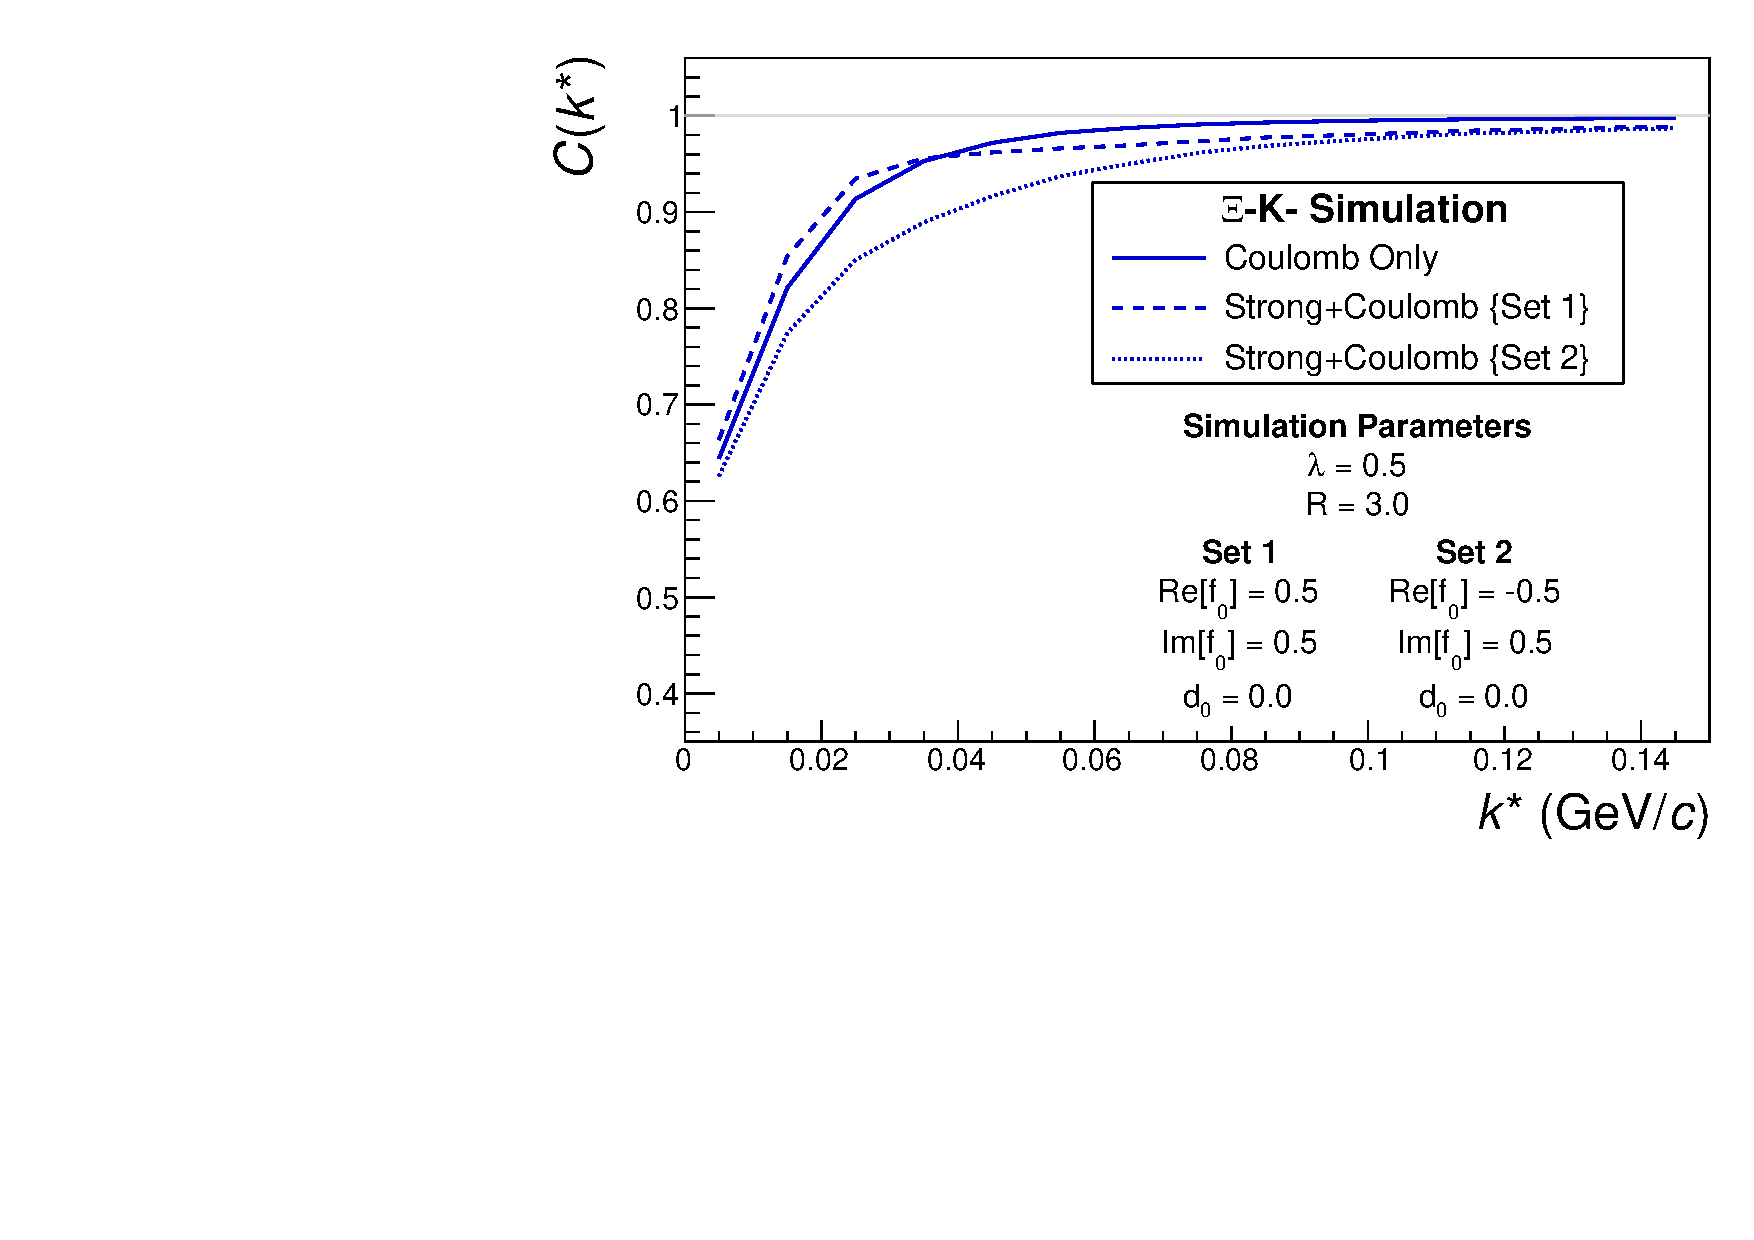
\includegraphics[width=0.99\textwidth]{7_ResultsAndDiscussion/Figures/WPCFStrongInfluence_XiKchM_0010_v2.pdf}}
  %%----overall caption----
  \caption[$\Xi$K$^{\pm}$ Coulomb Only]{$\Xi$K$^{\pm}$ Coulomb Only, 0-10\% Centrality}
  \label{fig:XiKchStrongInfluence}
\end{figure}


\begin{figure}[h]
  \centering
  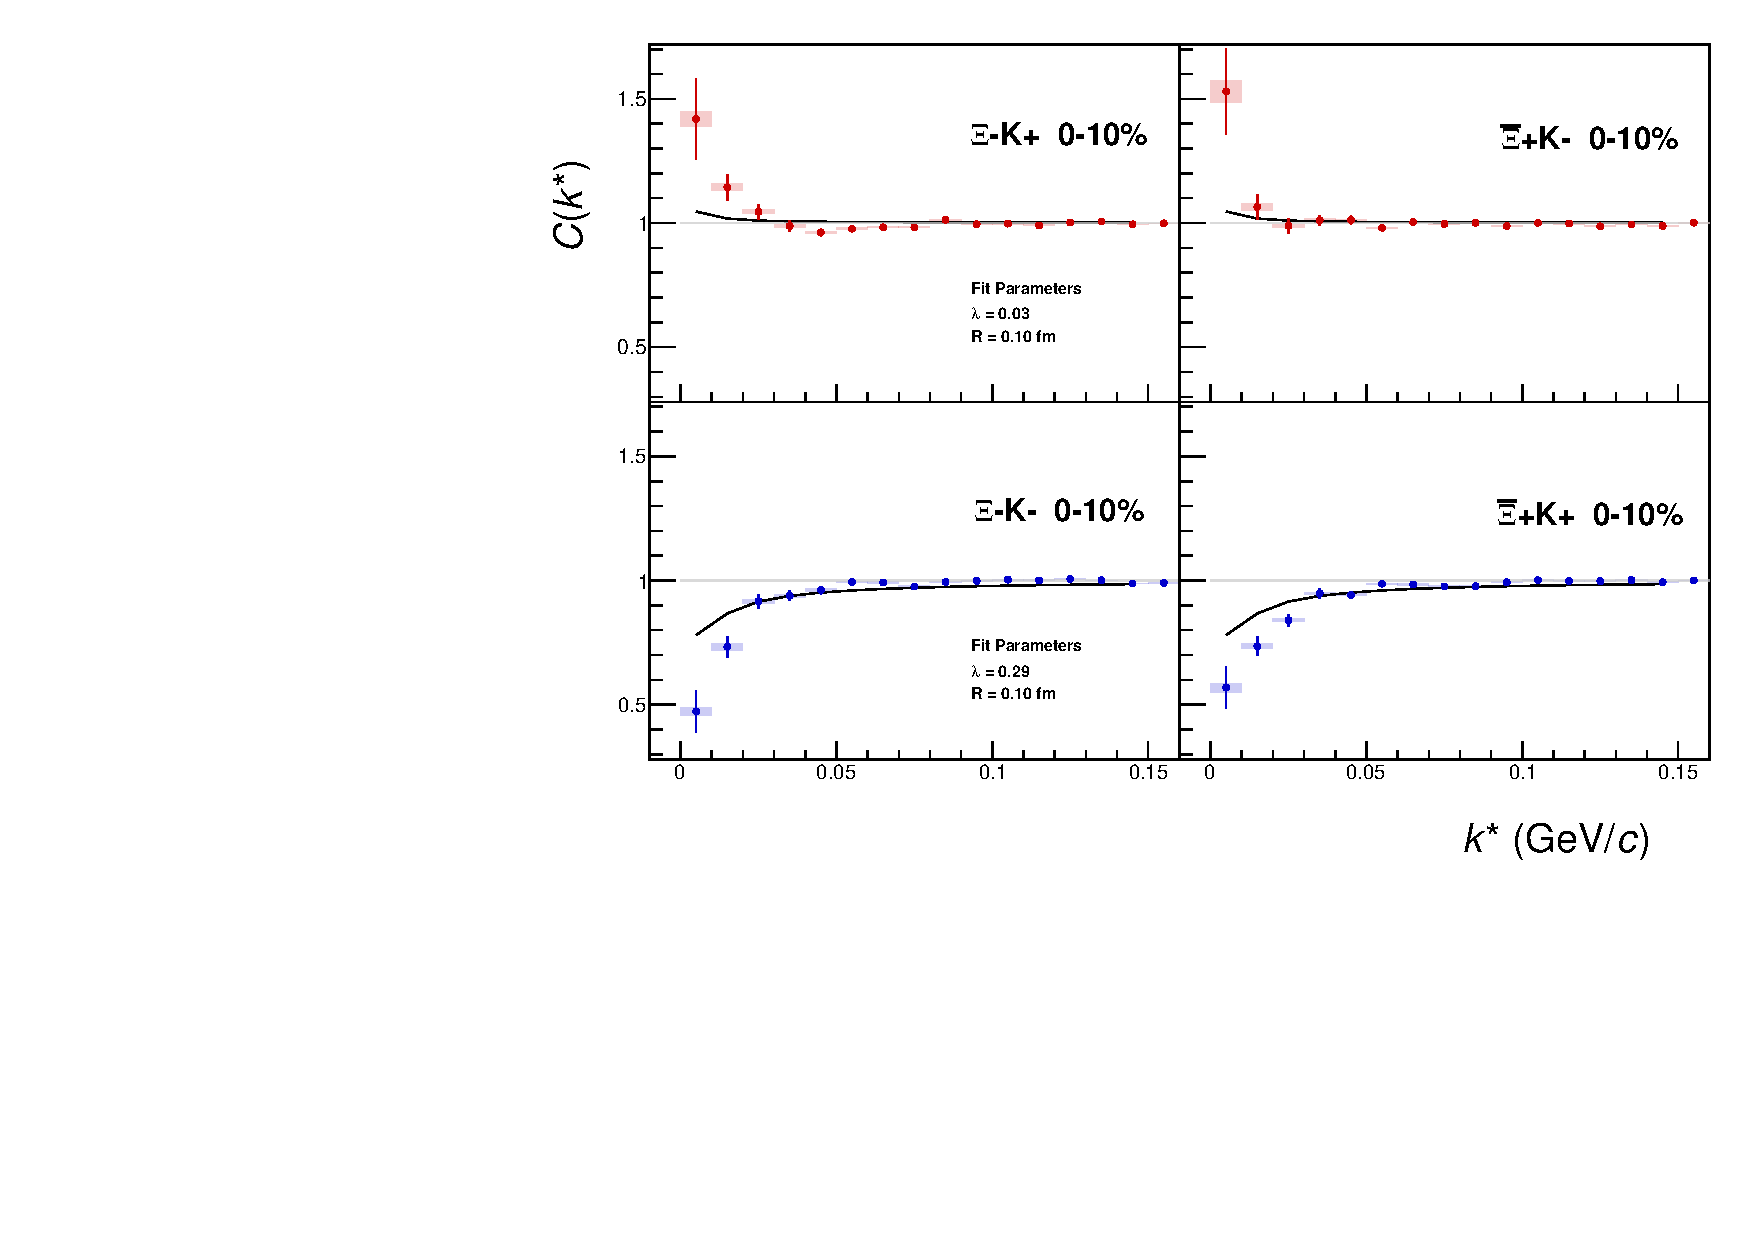
\includegraphics[width=\textwidth]{7_ResultsAndDiscussion/Figures/GlobalCoulombOnlyFit_Set1.pdf}
  \caption[$\Xi$K$^{\pm}$ Global Coulomb Only Fit (Set 1)]{$\Xi$K$^{\pm}$ Global Coulomb only fit (Set 1) for 0-10\% Centrality}
  \label{fig:XiKchGlobalCoulombOnlySet1}
\end{figure}

\begin{figure}[h]
  \centering
  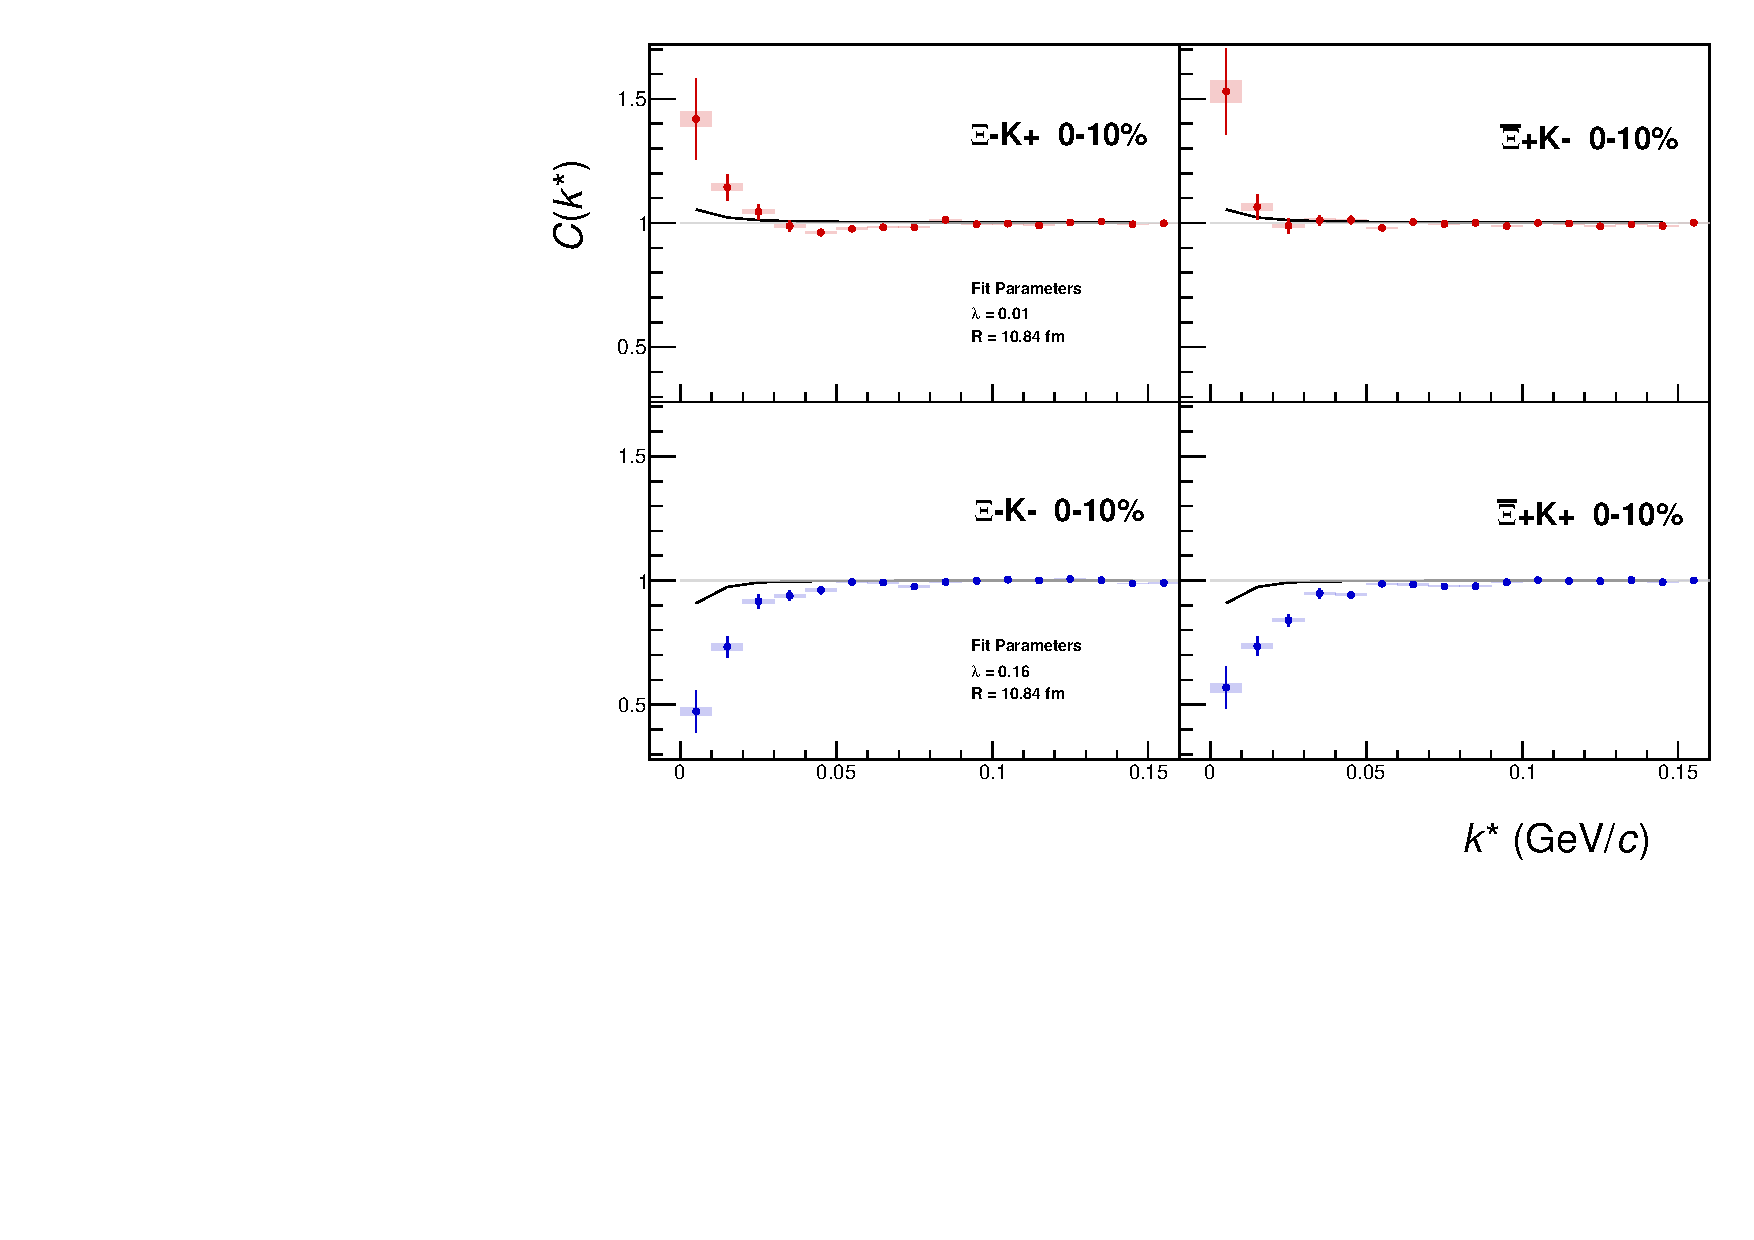
\includegraphics[width=\textwidth]{7_ResultsAndDiscussion/Figures/GlobalCoulombOnlyFit_Set2.pdf}
  \caption[$\Xi$K$^{\pm}$ Global Coulomb Only Fit (Set 2)]{$\Xi$K$^{\pm}$ Global Coulomb only fit (Set 2) for 0-10\% Centrality}
  \label{fig:XiKchGlobalCoulombOnlySet2}
\end{figure}

\begin{figure}[h]
  \centering
  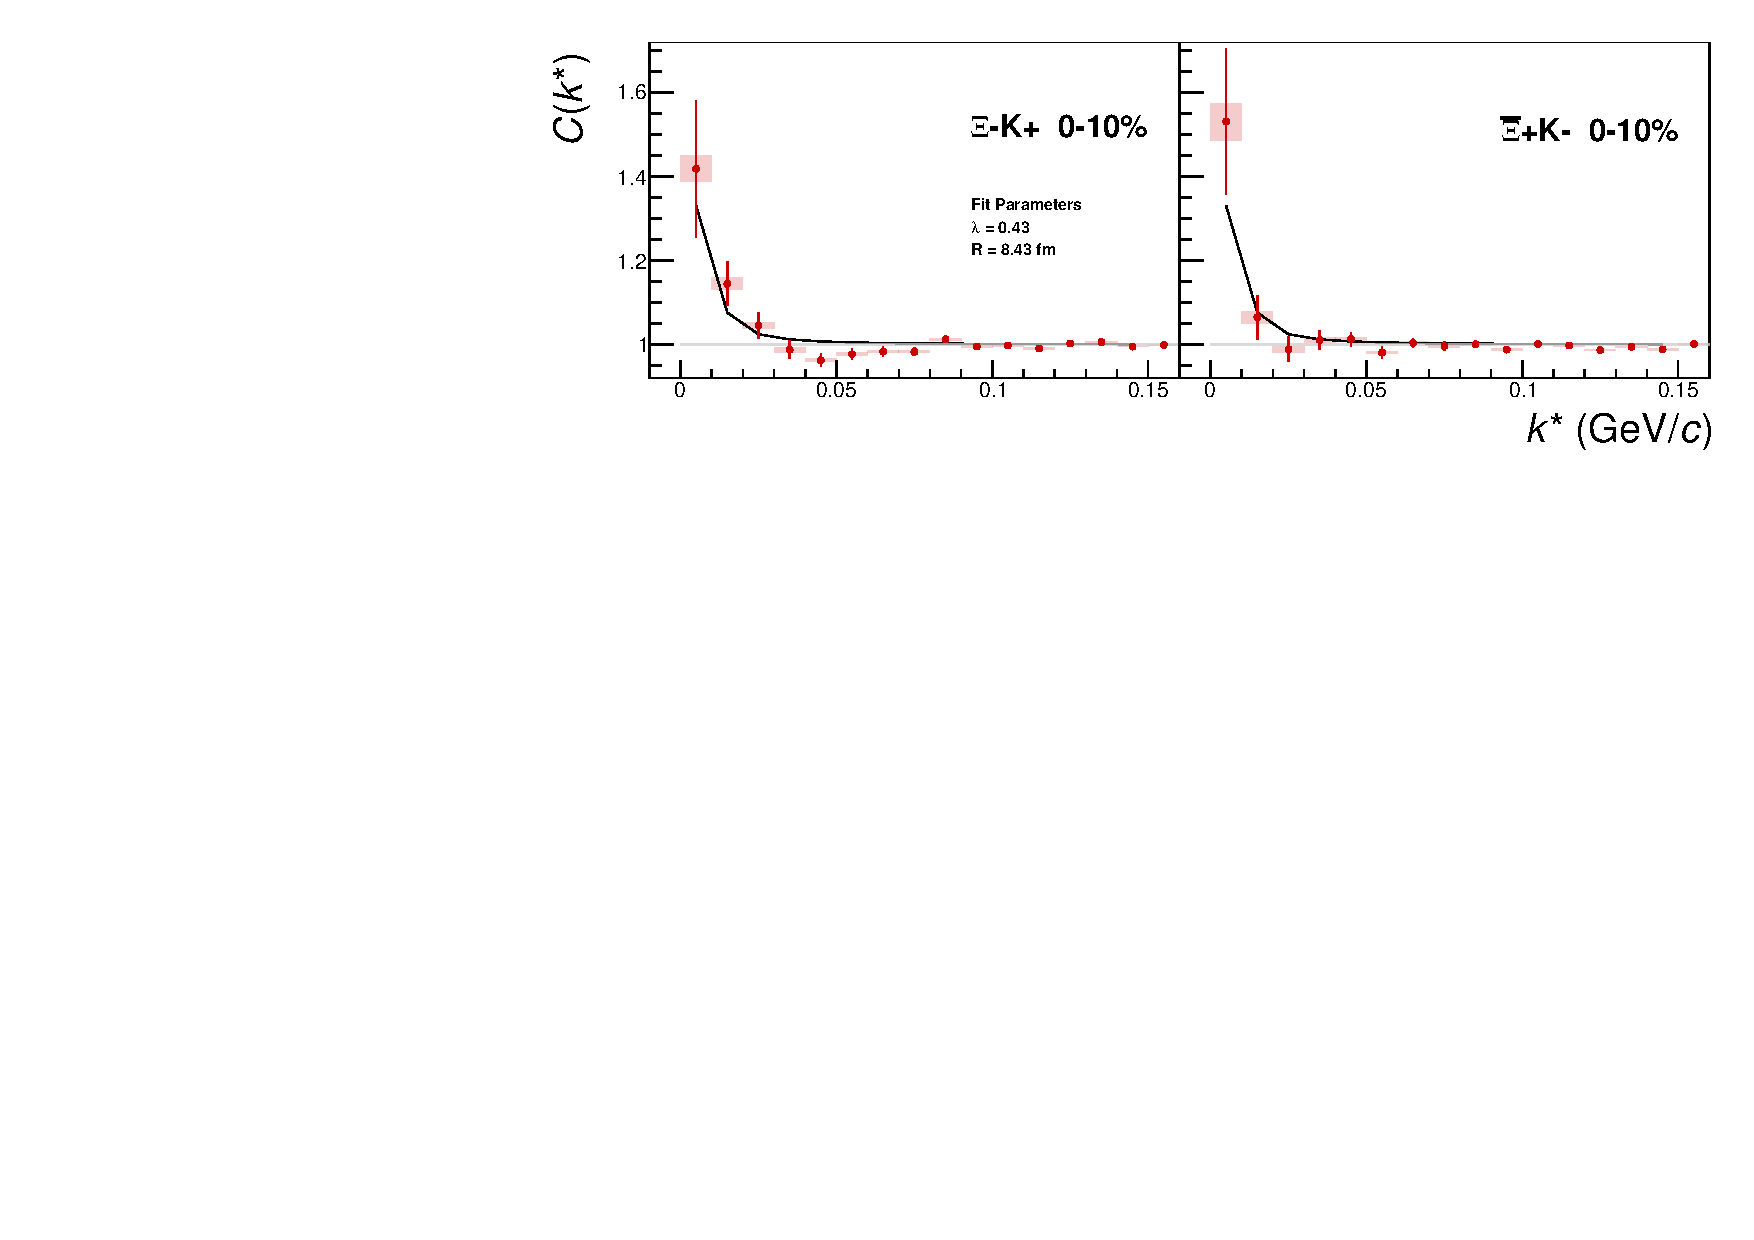
\includegraphics[width=\textwidth]{7_ResultsAndDiscussion/Figures/CoulombOnlyFitXiKchP_0010.pdf}
  \caption[$\Xi^{-}$K$^{+}$ Coulomb Only Fit]{$\Xi^{-}$K$^{+}$ Coulomb only fit for 0-10\% Centrality}
  \label{fig:XiKchPCoulombOnlyFit}
\end{figure}

\begin{figure}[h]
  \centering
  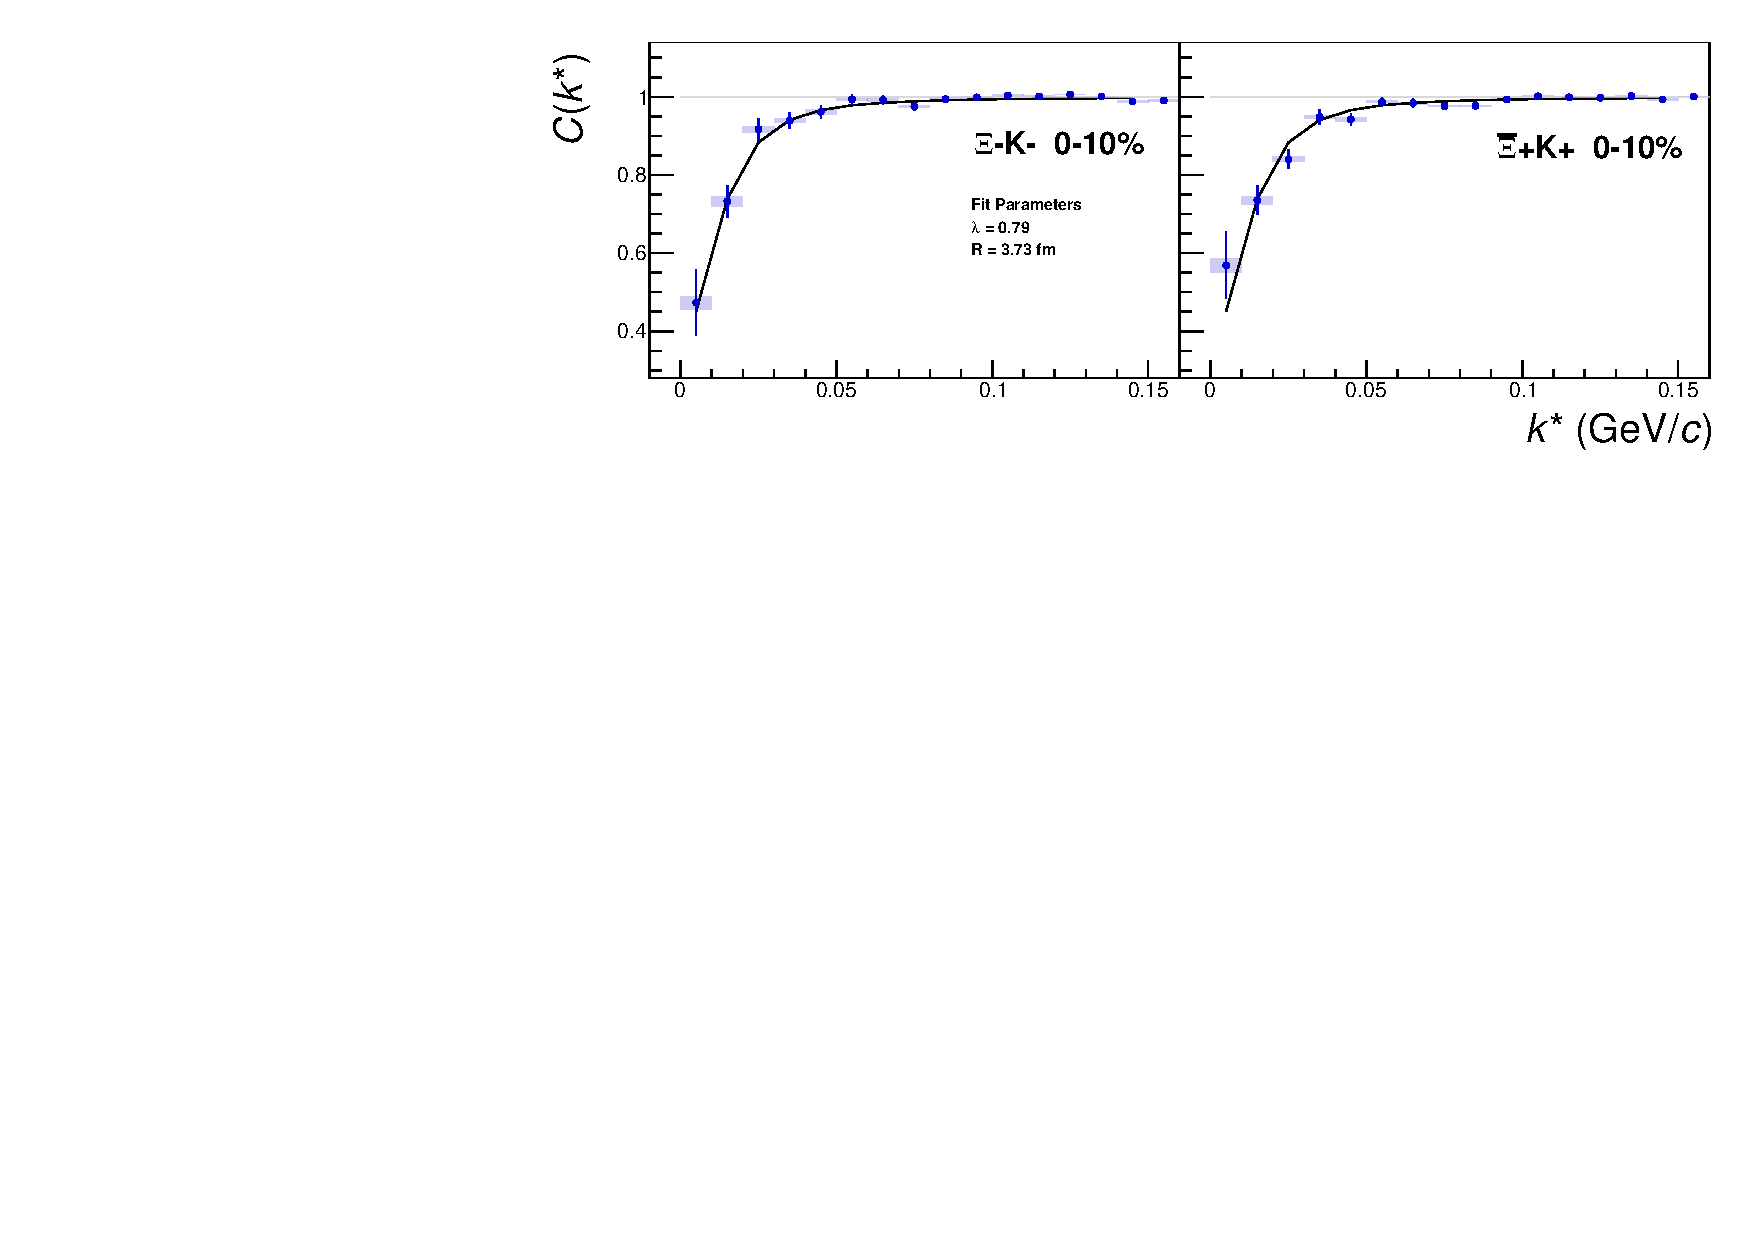
\includegraphics[width=\textwidth]{7_ResultsAndDiscussion/Figures/CoulombOnlyFitXiKchM_0010.pdf}
  \caption[$\Xi^{-}$K$^{-}$ Coulomb Only Fit]{$\Xi^{-}$K$^{-}$ Coulomb only fit for 0-10\% Centrality}
  \label{fig:XiKchMCoulombOnlyFit}
\end{figure}


\end{document}